\section{Evaluation}
\begin{frame}{Evaluation}
	
	\begin{itemize}
		\item Main goal of the platform is to simplify and automize the benchmark process of triplestores
		
		\item Evaluation of the added value to the benchmark process
		\begin{itemize}
			\item Using TENTRIS and Oxigraph triplestores
			
			\item Pulling official images from Docker Hub
			
			\item Comparing the manual benchmark process to the Basilisk process
		\end{itemize}
		
	\end{itemize}
	
	
\end{frame}

\begin{frame}{Comparison}
	
	\begin{columns}[T]
		\column{0.5\textwidth}
		\heading{Manual Process}
		\begin{enumerate}
			\item Finding initial benchmark setup
			\begin{itemize}
				\item Setting up triplestore in Docker container
				\item Loading dataset
				\item Configuring IGUANA framework
				\item Executing benchmark
			\end{itemize}
		
			\vspace{.85cm}
			\item Executing further benchmarks
			\begin{itemize}
				\item Repeat same manual steps
			\end{itemize}
			
		\end{enumerate}
		
		
		\column{0.5\textwidth}
		\heading{Basilisk Process}%\vspace*{.2cm}
		\begin{enumerate}
			\item Finding initial benchmark setup
			\begin{itemize}
				\item Setting up triplestore in Docker container
				\item Loading dataset
				\item Configuring IGUANA framework
				\item Executing benchmark
				\item Transfer configuration to Basilisk platform
			\end{itemize}
		
			\item Executing further benchmarks
			\begin{itemize}
				\item Automated through platform
				\item Starting a manual job
			\end{itemize}
		\end{enumerate}
	\end{columns}
	
\end{frame}

\begin{frame}{Evaluation}
	\begin{itemize}
		\item Using the platform multiple benchmarks were performed using the Semantic Web Dog Food (SWDF) benchmark
		\begin{itemize}
			\item Benchmarked 16 versions of TENTRIS
			\item 9 versions of Oxigraph
		\end{itemize}
	\end{itemize}
	
	\centering
	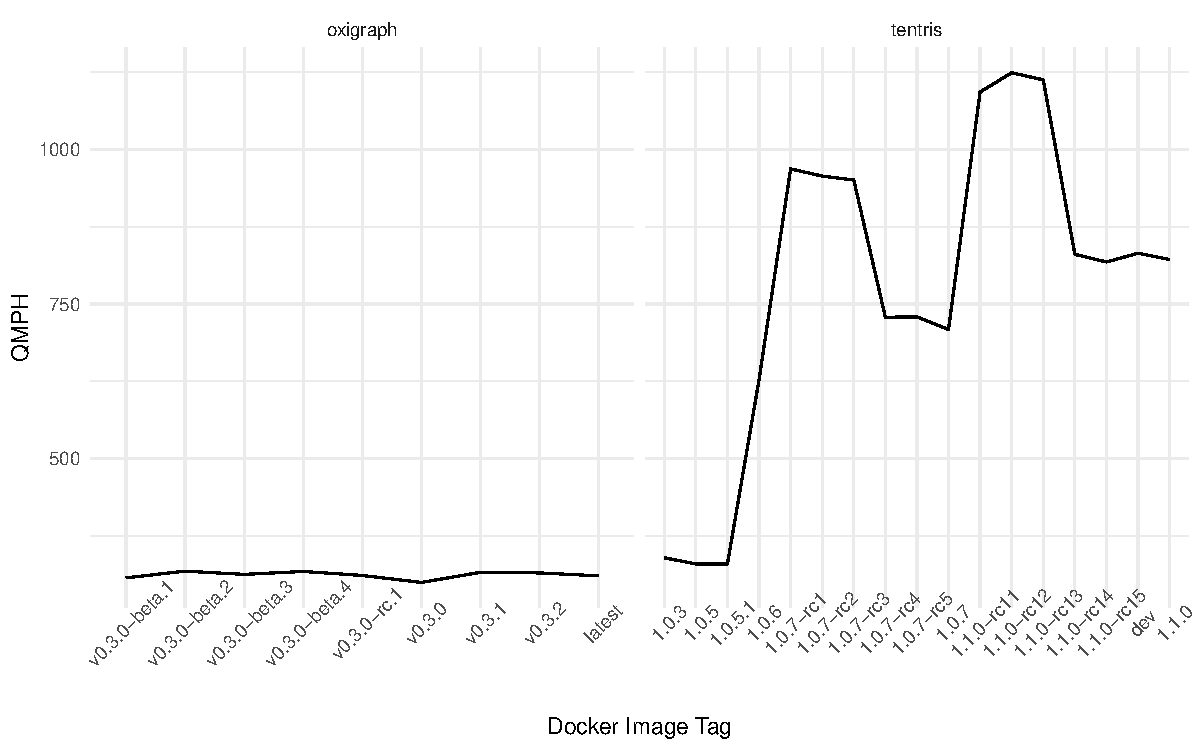
\includegraphics[width=.8\textwidth]{images/basilisk/QMPH.pdf}
\end{frame}

